In this chapter, we provide a proof of concept of Blockchain-based Federated Learning (BFS) applied to a system with vertically partitioned data. With this experiments, we want to show that:

\begin{enumerate}
    \item It is possible to implement a Blockchain-based Vertical Federated Learning. As discussed in \Cref{related_work:other_remarks}, only one other work argues that it is possible to implement such system, but provides no description or code of their framework.

    \item It is possible to have a BFL framework that supports both Horizontal Federated Learning and Vertical Federated Learning. One of the goals of this thesis is to build a modular framework that can be easily adapted to support multiple techniques and algorithms.
    
    \item Our framework is flexible enough to support additional phases and techniques. As explained in \Cref{eval:ml_models}, the model we use for Vertical Federated Learning requires an additional step in each round. By showing that it is trivial to add new steps to the rounds, we also prove that BlockLearning is flexible.
\end{enumerate}

As discussed in \Cref{eval:ml_models}, our Vertical Federated Learning implementation uses the Split-CNN model. This model poses different requirements on our framework. In this section, we go over the requirements and how we can extend BlockLearning in order to successfully support the Split-CNN model.

\section{Split-CNN Requirements}

Firstly, we define which requirements the Split-CNN model has that are not yet satisfied by the BlockLearning framework:

\begin{enumerate}
    \item Different models for the clients and the servers. As explained in \Cref{eval:ml_models}, the clients have the head model, while the servers have the tail model.
    
    \item Additional backpropagation confirmation phase. After submitting the aggregations, and before terminating the round, the clients have to confirm that they backpropagated the model updates from the tail model to their own head models.
\end{enumerate}

The second requirement can be further subdivided into the following functionalities:

\begin{enumerate}
    \item Backpropagation confirmation phase executes after aggregations submission phase.

    \item Backpropagation gradient submission by the servers to the smart contract.
    
    \item Backpropagation retrieval by the clients from the smart contract.
    
    \item Backpropagation confirmation by the clients to the smart contract.
\end{enumerate}

\section{BlockLearning Extension}

Most of the requirements aforementioned pertain the smart contract. Therefore, we first start by adding a new phase to the \texttt{RoundPhase} enumeration, and creating a new smart contract, \texttt{VerticalSplitCNN}. The smart contract provides additional functionality in order to support the new backpropagation confirmation phase. \autoref{fig:uml-vertical} illustrates the smart contract additions when compared to the original design depicted in \autoref{fig:contracts-uml}.

\begin{figure}[!ht]
    \centering
    \centering
    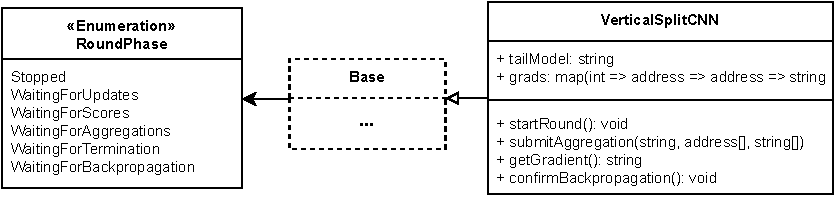
\includegraphics[width=1\textwidth]{graphics/smart-contract-uml-vertical.pdf}
    \caption{Split-CNN Smart Contracts Extension Class Diagram}
    \label{fig:uml-vertical}
\end{figure}

After creating the new smart contract, the smart contract bridge has to be extended in order to include the new smart contract functions. This extension is trivial as explained in \Cref{impl:bridge}.

The model training procedure is also slightly different as we share, not the weights, but the intermediate output of the last layer of the head models. Therefore, we implement a new \texttt{TrainerSplitCNN} class that supports both the methods \texttt{train()} and \texttt{backward()}.

Finally, we create a Server and Client scripts using the BlockLearning framework. \autoref{alg:client_loop_splitcnn} illustrates how the client script main loop works when working with the Split-CNN. The main differences when compared to the regular client loop we saw in \autoref{alg:client_loop} is that it does not include a scoring algorithm and checks for an additional phase.

\begin{algorithm}
\caption{Client Script Main Loop for Split-CNN}\label{alg:client_loop_splitcnn}
\begin{algorithmic}
\State $T \gets $ Initialize Trainer
\While{True}
    \State $P \gets$ Get Phase From Smart Contract
    \If{$P$ is Waiting For Updates}
        \State Execute Training Procedure $T.train()$
    \ElsIf{$P$ is Waiting For Backpropagation}
        \State Execute Backpropagation Procedure $T.backward()$
    \EndIf
\EndWhile
\end{algorithmic}
\end{algorithm}

\section{Executing the Experiment}

% This experiment was performed with two different number of clients: 2 and 4, with a dual-headed, and four-headed Split-CNN model, respectively. In addition, most Vertical Federated Learning models from the literature were applied to 2 clients. Therefore, it is interesting to see that it is possible to easily apply the model to more clients.

% \section{Execution Time, Transaction Cost, and Transaction Latency}

% The execution time and transaction metrics can be seen in \autoref{tab:metrics_vertical}. It is observable that the more the clients, the longer a round takes to be completed. As such the entire learning process takes longer. This is a conclusion that was taken in a previous chapters, too.

% Regarding the transaction latency and cost, we can see that both are similar to what has been seen in previous chapters. Since the number of clients is low, we did not expect to have significant differences in either of them.

% \begin{table}[!ht]
% \begin{tabular}{c|c|c} \hline \hline
%                                 & 2             & 4             \\ \hline \hline
% E2E Time (m)                    & 10.97	        & 12.57         \\ \hline
% Mean Round Time (s)             & 13.16	        & 15.08         \\ \hline
% Mean Transaction Latency (s)    & 1.642	        & 1.546         \\ \hline
% Mean Transaction Cost (Gas)     & 141335        & 142638        \\ \hline
% \end{tabular}
% \caption{Execution Time, Transaction Cost, and Transaction Latency Per Number of Clients}
% \label{tab:metrics_vertical}
% \end{table}

% \section{Accuracy and Convergence}

% Regarding accuracy, we can observe smooth convergences, as well as similar high accuracy. Both clients reached an accuracy above $85\%$, only differing in $3\%$. In addition, it is interesting to see that the convergence of the Vertical Federated Learning is much smoother than what we have observed with Horizontal Federated Learning. This is likely explained by the fact that in this setting, all clients participate in each round due to the way the data is structured. In addition, the model is different from a regular CNN, which may lead to different results. However, since both types of data partition solve different types of problems, it is not a fair comparison.

% \begin{figure}[!ht]
%     \centering
%     \centering
%     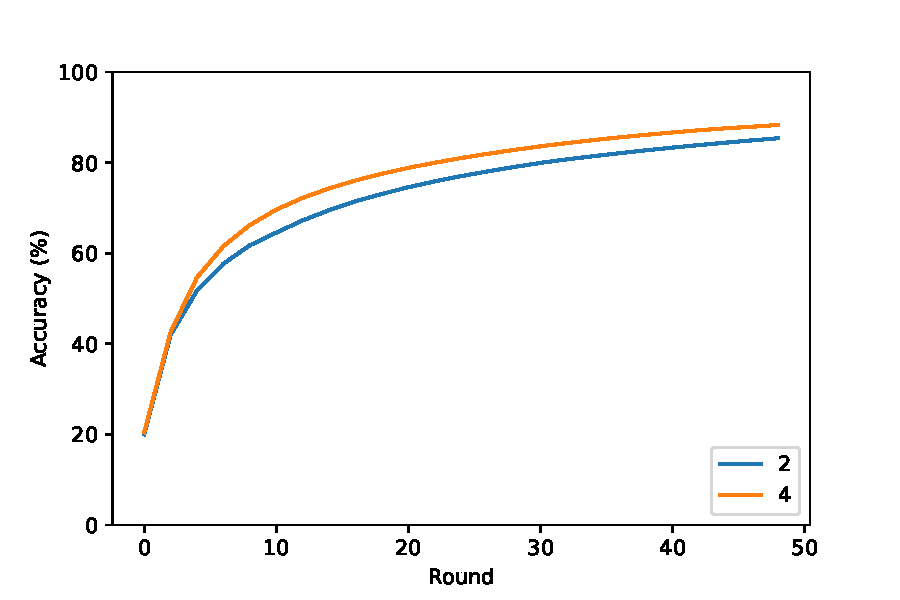
\includegraphics[width=0.7\textwidth]{graphics/vertical/accuracy.pdf}
%     \caption{Accuracy Per Number of Clients}
%     \label{fig:accuracy_vertical}
% \end{figure}

% \section{Communication Costs}

% The communication costs represented in \autoref{fig:net_vertical} are also within the expected values.

% On the clients, we can observe that there is no major difference of traffic when the number of clients increases. This can be explained by the fact that, by using a Split-CNN, each client is only required to upload their own intermediate results and download the gradient updates, which have fixed sizes.

% On the servers, the costs are higher with more clients. Since the Split-CNN model has more heads with more clients, the servers are required to download more intermediate results, as well as upload more gradient updates. Therefore, it would be expected that the traffic would double with the double of clients.

% On the blockchain, the difference of amount of clients is not significant to make a significant difference on traffic.

% \begin{figure}[!ht]
%     \centering
%     \centering
%     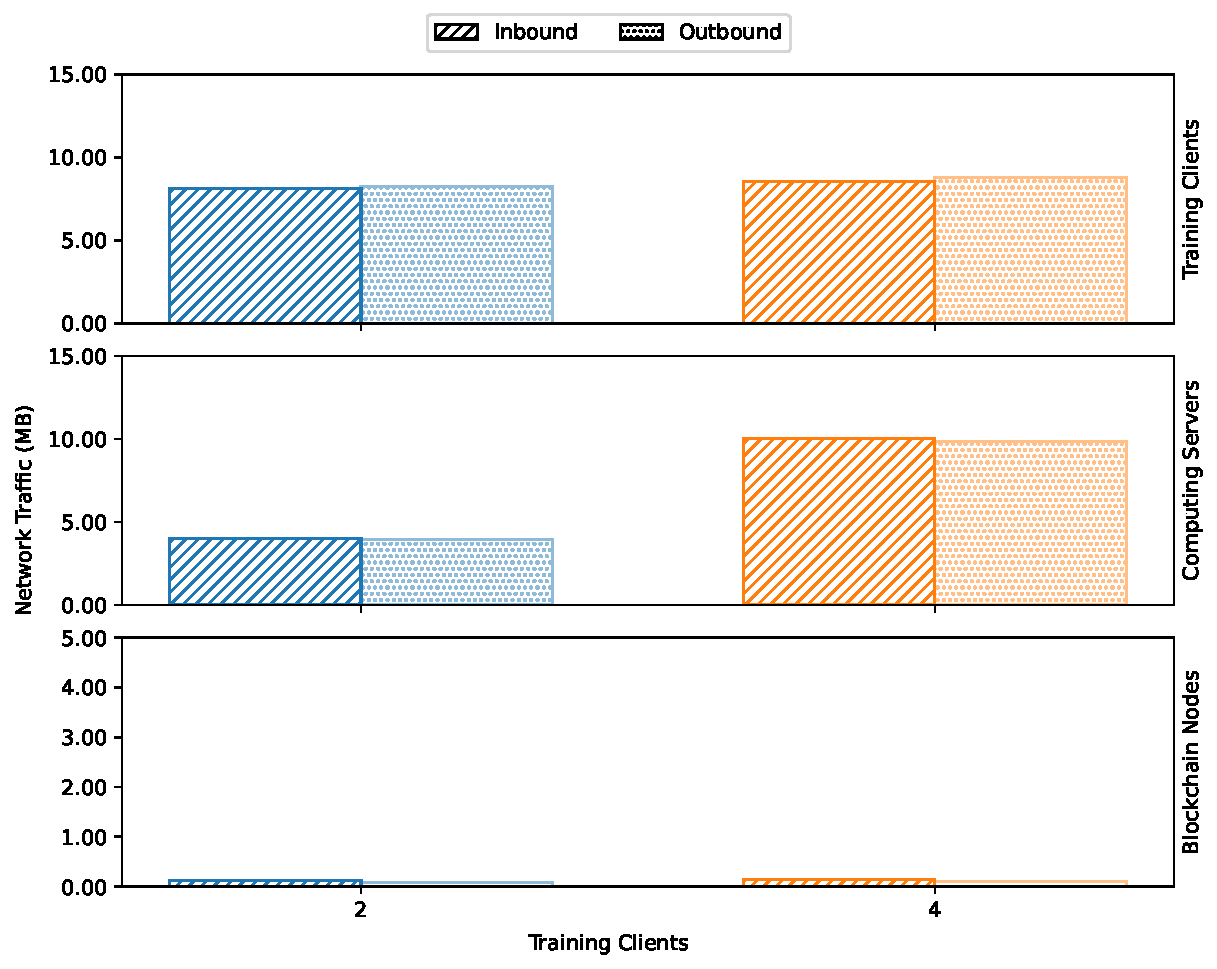
\includegraphics[width=0.8\textwidth]{graphics/vertical/net.pdf}
%     \caption{Network Traffic Per Round Per Number of Clients}
%     \label{fig:net_vertical}
% \end{figure}

% \section{Computation Costs}

% Computation costs, namely RAM usage and CPU usage, are depicted in \autoref{fig:ram_vertical} and \autoref{fig:cpu_vertical}, respectively. As expected, with higher amounts of clients there is a slightly higher RAM consumption on both the server and blockchain processes, caused by more data being stored in-memory, as well as more messages being carried over the blockchain. However, we see the opposite happening with the clients. This is explained by the fact that the dual-headed CNN contains an additional convolutional layer compared to the four-headed CNN, which leads to more RAM usage during training. Regarding CPU usage, we see similar results as to the RAM usage, which are explained by the same reasons.

% \begin{figure}[!ht]
%     \centering
%     \centering
%     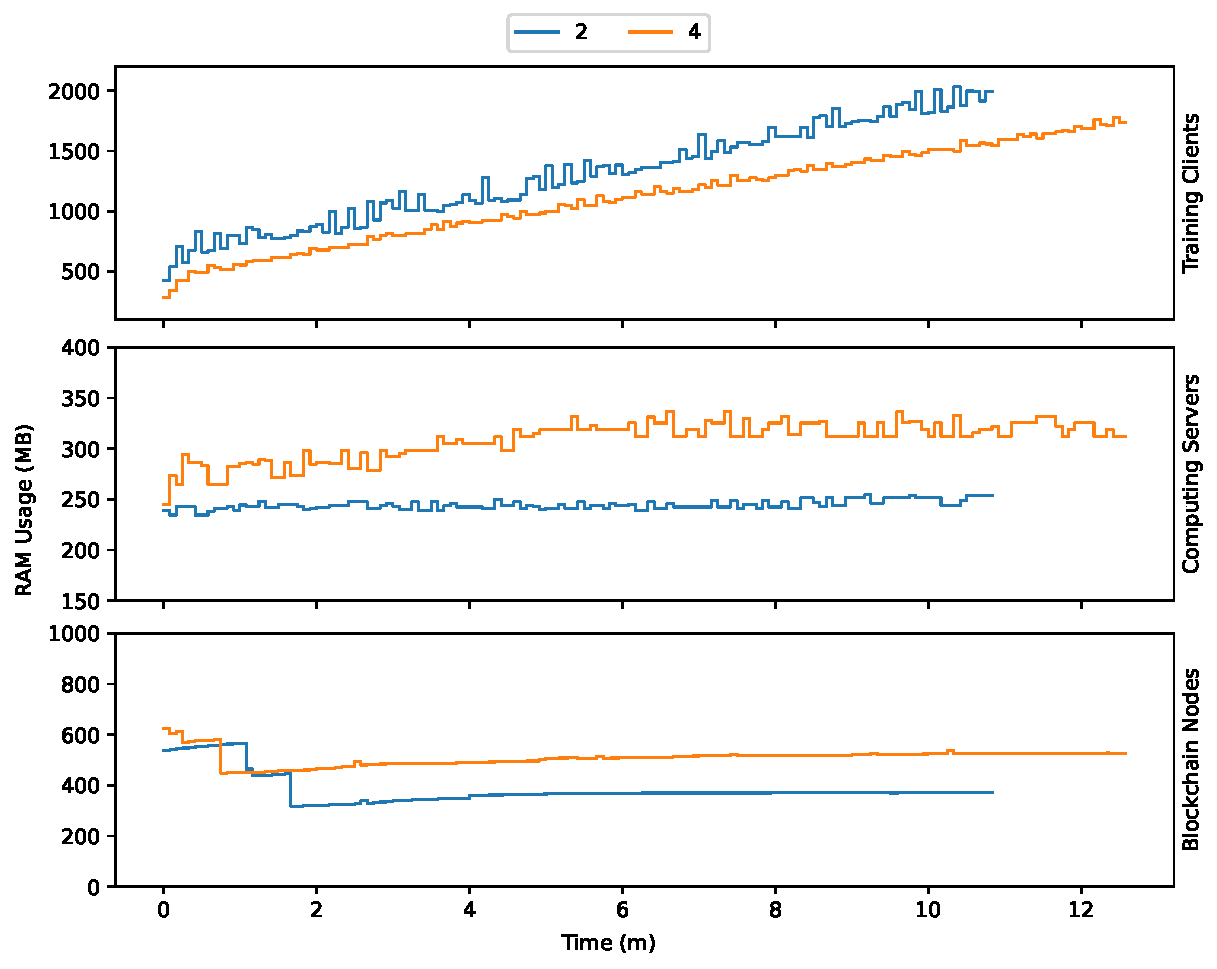
\includegraphics[width=0.8\textwidth]{graphics/vertical/ram.pdf}
%     \caption{RAM Usage Per Number of Clients}
%     \label{fig:ram_vertical}
% \end{figure}

% \begin{figure}[!ht]
%     \centering
%     \centering
%     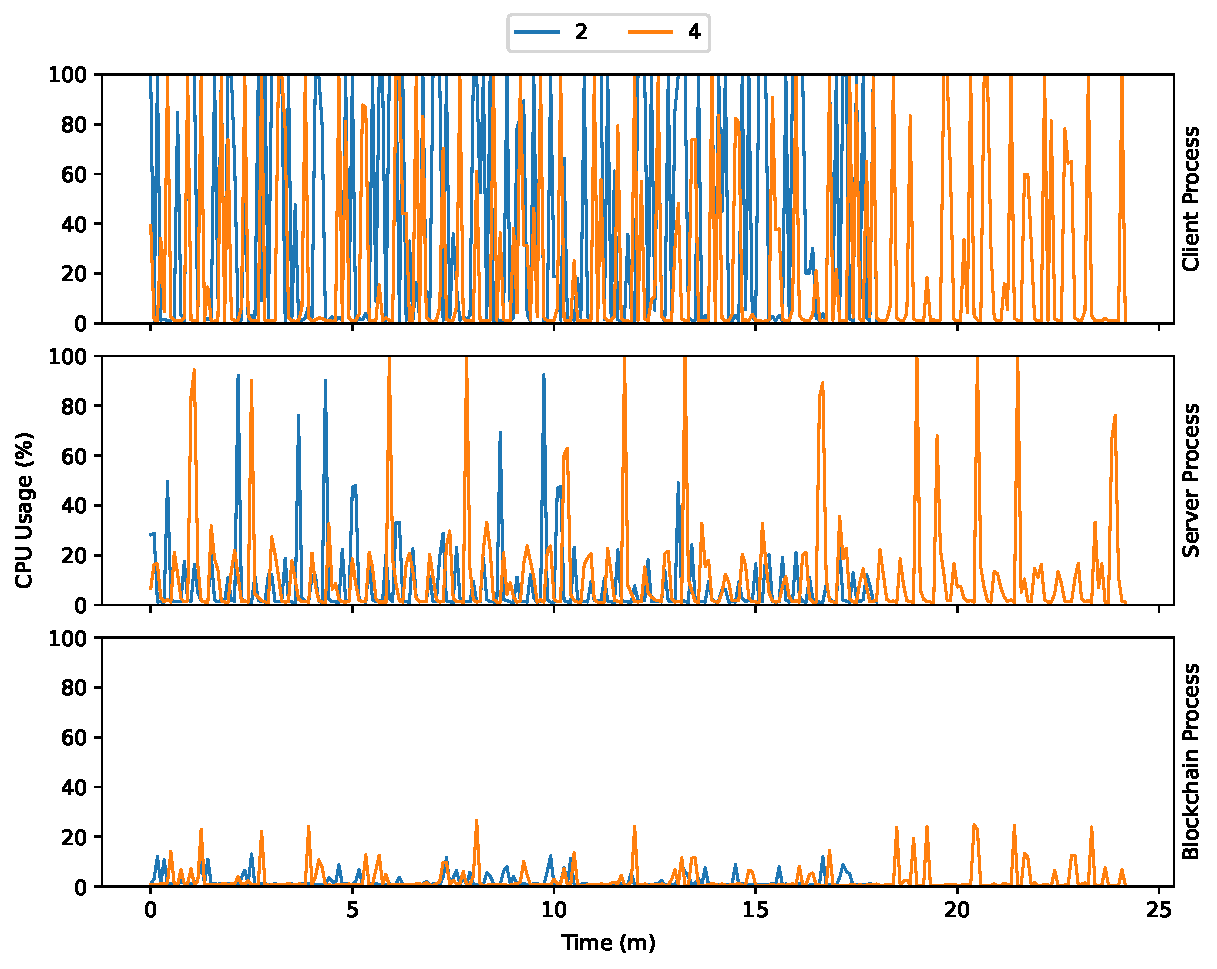
\includegraphics[width=0.8\textwidth]{graphics/vertical/cpu.pdf}
%     \caption{CPU Usage Per Number of Clients}
%     \label{fig:cpu_vertical}
% \end{figure}

\section{Conclusions and Improvements}

% From this experiment, we can conclude that it is possible to apply a Blockchain-based Federated Learning system to vertically partitioned data. In future work, it would be interesting to investigate how to apply other models. In addition, it would be interesting to see how other, larger data sets, could be applied with larger amounts of clients. Using MNIST, this experiment is limited because of the extremely small resolution of the images. Therefore, it is not feasible to separate many features. Finally, it would also be worth investigating how privacy mechanisms could be applied to the intermediate model outputs in order to prevent inference attacks.
